\chapter{Задание 2. Линейные фильтры}
\label{ch:chap2}

\definecolor{codegreen}{rgb}{0,0.6,0}
\definecolor{codegray}{rgb}{0.5,0.5,0.5}
\definecolor{codepurple}{rgb}{0.58,0,0.82}
\definecolor{backcolour}{rgb}{0.95,0.95,0.92}

\lstdefinestyle{mystyle}{
    backgroundcolor=\color{backcolour},   
    commentstyle=\color{codegreen},
    keywordstyle=\color{magenta},
    numberstyle=\tiny\color{codegray},
    stringstyle=\color{codepurple},
    basicstyle=\ttfamily\footnotesize,
    breakatwhitespace=false,         
    breaklines=true,                 
    captionpos=b,                    
    keepspaces=true,                 
    numbers=left,                    
    numbersep=5pt,                  
    showspaces=false,                
    showstringspaces=false,
    showtabs=false,                  
    tabsize=2
}
\lstset{style=mystyle}

Возьмём шумный сигнал из прошлой лабы, но будем применять оружие покрупнее:
$$
\texttt{u = g + b*(rand(size(t))-0.5) + c*sin(d*t);}
$$

\section{Фильтр первого порядка}
Линейный фильтр первого порядка мы зададим следующим образом:
$$ W_1(p)=\frac{1}{Tp + 1}$$

Берём $d=c=0$, также зададим постоянную времени $T > 0$ для фильтра. Тогда в этом пункте мы будем работать со следующей версией шумного сигнала:
$$\texttt{u = g + b*(rand(size(t))-0.5)}$$
\dots из чего сразу следует, что у нас добавляется только "случайный" шум.

\subsection{Испытания}
Построим сравнительные графики исходного и фильтрованного сигналов, графики модулей их Фурье-образов, а также АЧХ  и ФЧХ фильтра. 
Чтобы возможно упростить общий анализ, я свёл все эти графики в подграфики.


\begin{figure}[ht]
    \centering
    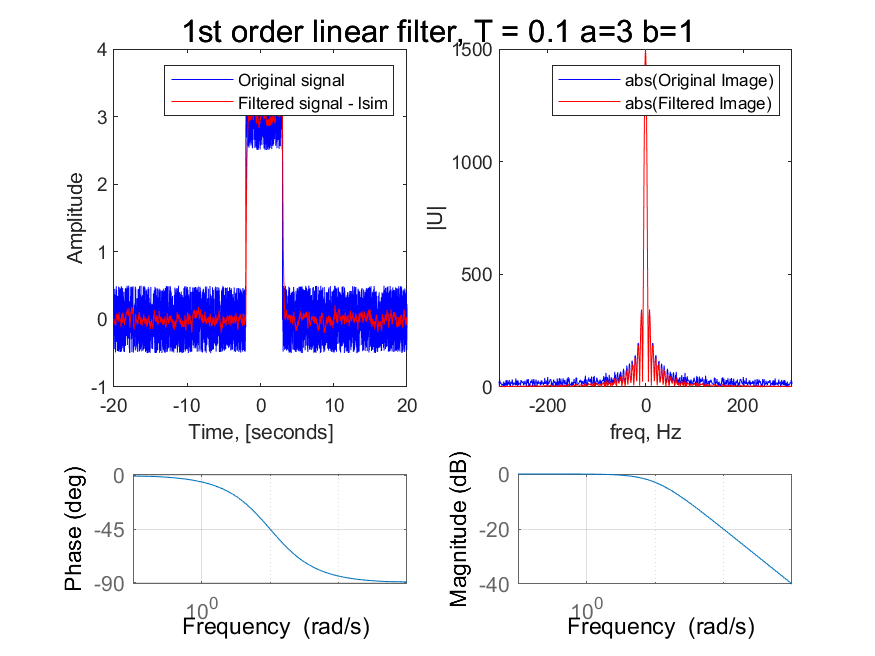
\includegraphics[width=1\textwidth]{test_linear_filter=3_b=1_T=0_10.png}
	\caption{Испытание 1}
\end{figure}

\begin{figure}[ht]
    \centering
    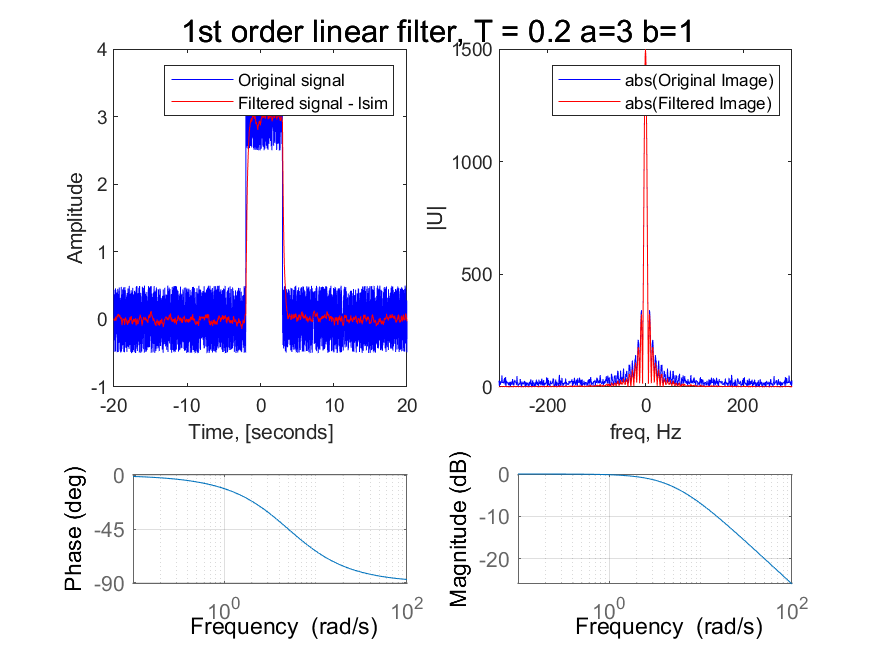
\includegraphics[width=1\textwidth]{test_linear_filter=3_b=1_T=0_20.png}
	\caption{Испытание 2}
\end{figure}

\begin{figure}[ht]
    \centering
    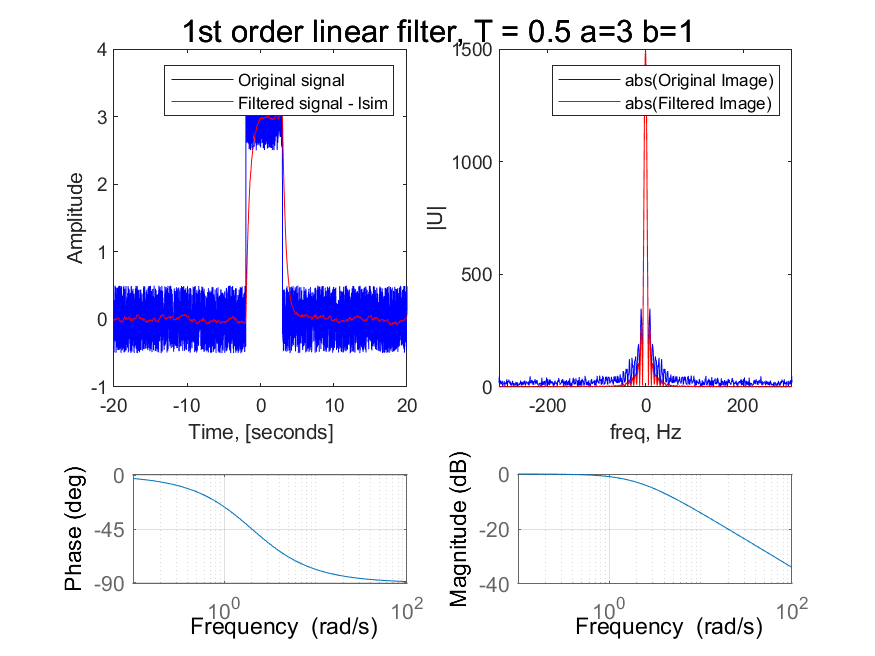
\includegraphics[width=1\textwidth]{test_linear_filter=3_b=1_T=0_50.png }
	\caption{Испытание 3}
\end{figure}
\newpage
\begin{figure}[ht]
    \centering
    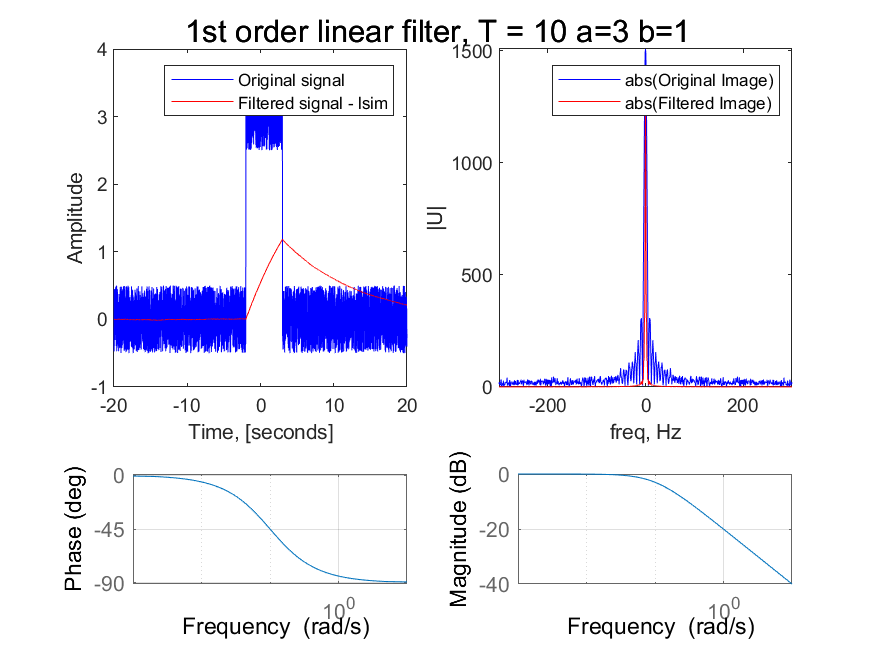
\includegraphics[width=1\textwidth]{test_linear_filter=3_b=1_T=10_00.png }
	\caption{Испытание 4}
\end{figure}

\begin{figure}[ht]
    \centering
    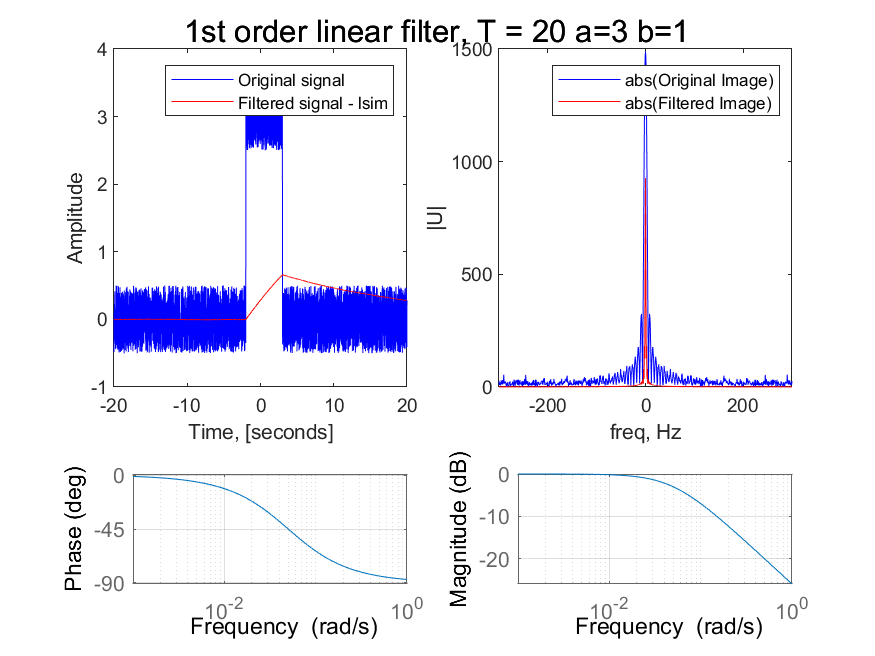
\includegraphics[width=1\textwidth]{test_linear_filter=3_b=1_T=20_00.png}
	\caption{Испытание 5}
\end{figure}
\newpage
\begin{figure}[ht]
    \centering
    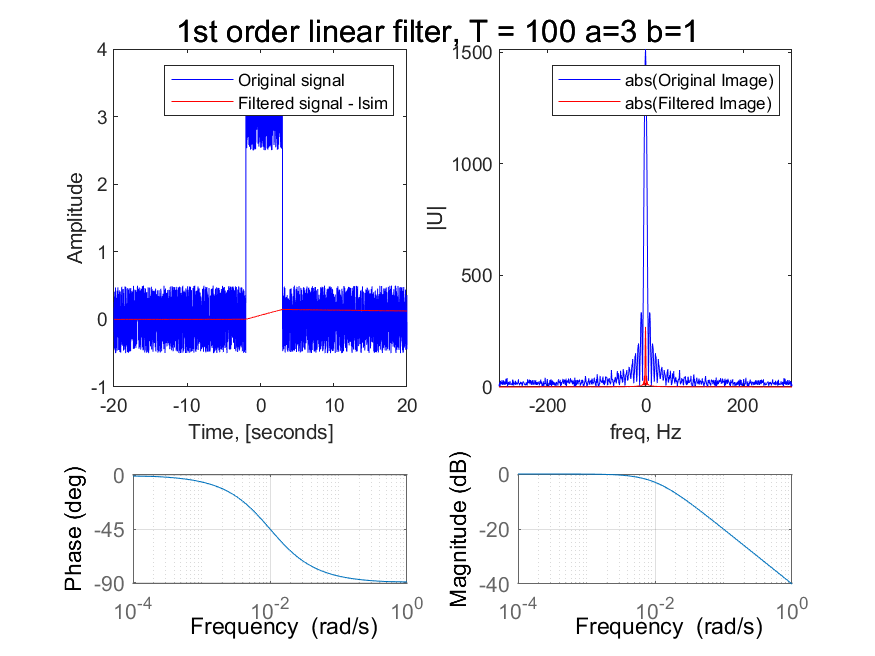
\includegraphics[width=1\textwidth]{test_linear_filter=3_b=1_T=100_00.png}
	\caption{Испытание 6}
\end{figure}

\begin{figure}[ht]
    \centering
    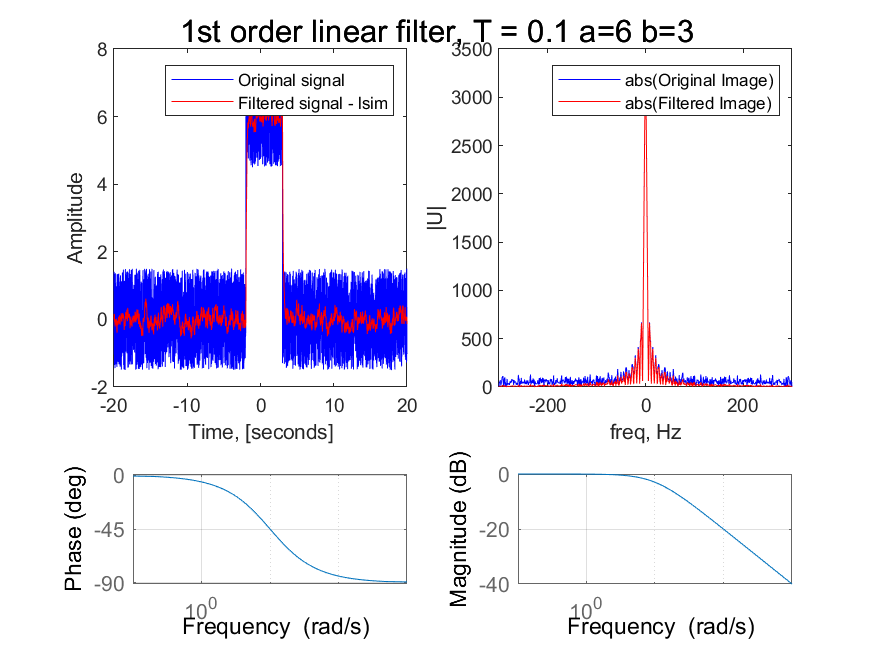
\includegraphics[width=1\textwidth]{test_linear_filter=6_b=3_T=0_10.png}
	\caption{Испытание 7}
\end{figure}
\newpage
\begin{figure}[ht]
    \centering
    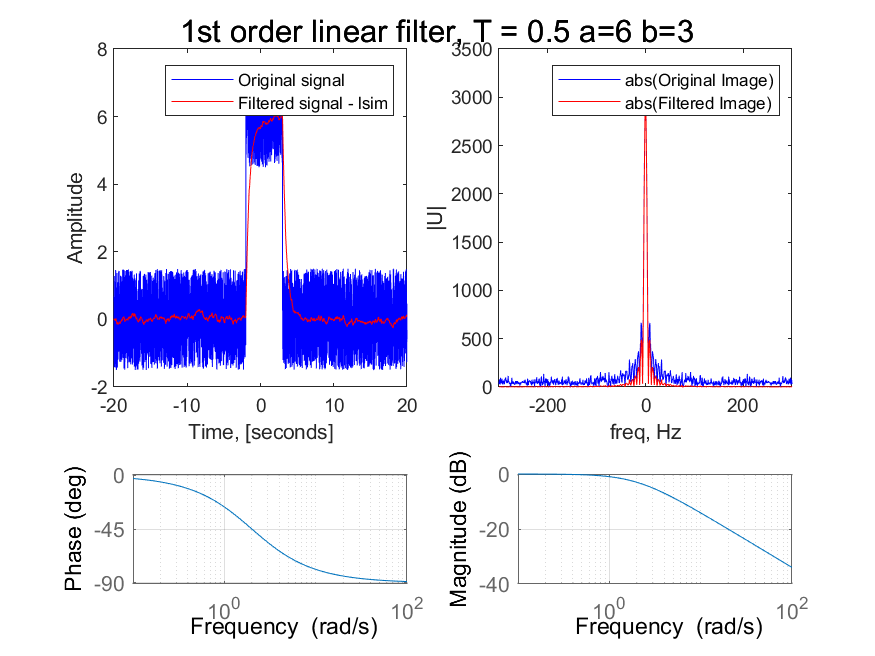
\includegraphics[width=1\textwidth]{test_linear_filter=6_b=3_T=0_50.png }
	\caption{Испытание 8}
\end{figure}

\begin{figure}[ht]
    \centering
    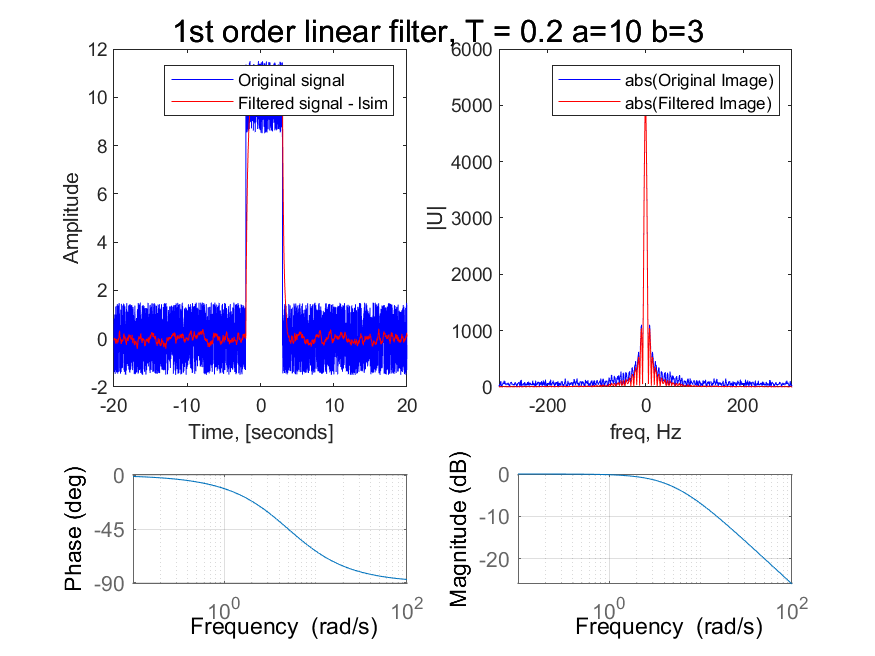
\includegraphics[width=1\textwidth]{test_linear_filter=10_b=3_T=0_20.png}
	\caption{Испытание 9}
\end{figure}


\newpage
\subsection{Выводы}
Давайте исследовать влияние постоянной времени $T$ и значения параметра $a$ на эффективность фильтрации. Возможно это не слишком заметно, но параметр $a$ у нас влияет на добавление белого шума и как бы мы не пытались увеличивать его амплитуду, - фильтр все равно более менее хорошо справлялся с таким шумом.
Но фильтр в первую очередь справлялся из-за хорошо подобранной постоянной времени - больше единицы ставить не было смысла, потому что результат плачевный. Поэтому подбирая на ощупь в пределах $[0 ; 1]$ с шагом $0.1$ можно было достичь приемлимых результатов.




\section{Специальный фильтр}
Выберем только $b=0$, остальные будут как-то заданы. Теперь мы уже имеем дело с двумя компонентами шума - случайным и гармоническим:
$$
\texttt{u = g + b*(rand(size(t))-0.5) + c*sin(d*t);}
$$
\subsection{Испытания}

\begin{figure}[ht]
    \centering
    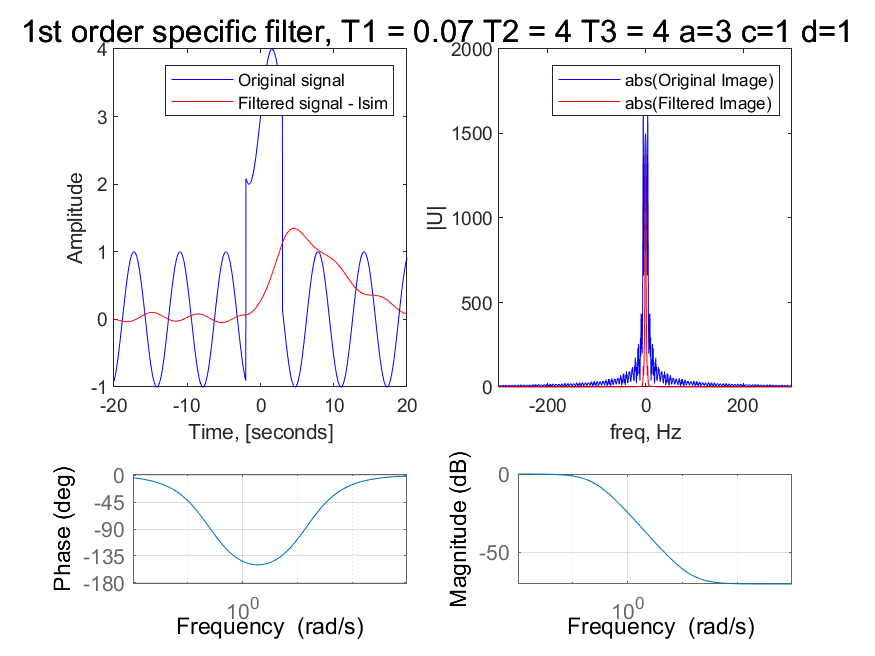
\includegraphics[width=1\textwidth]{test_specific_filter=3_b=0_c=1_d=1_T1=0_07_T2=4_00_T3=4_00.png}
	\caption{Испытание 1}
\end{figure}

\begin{figure}[ht]
    \centering
    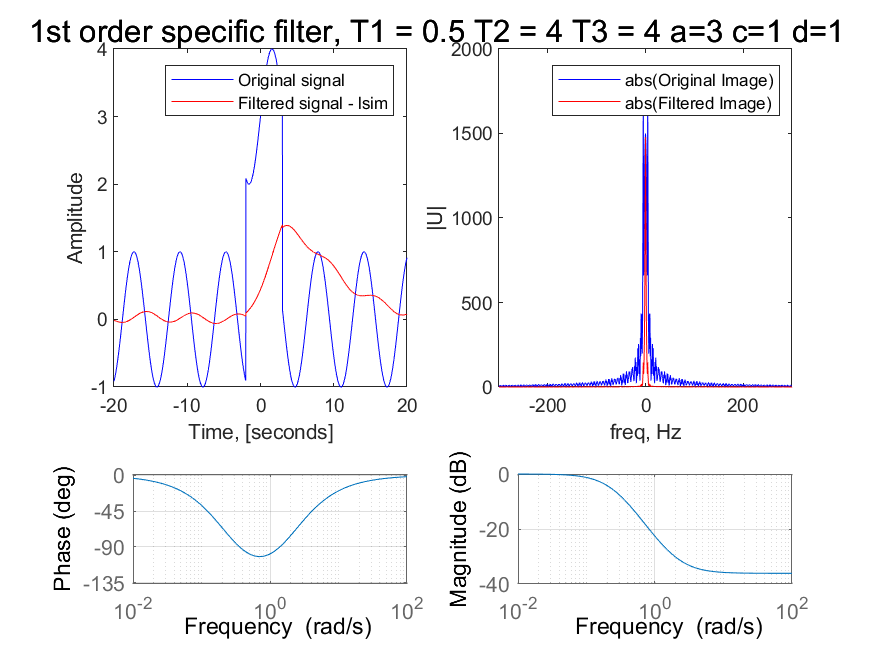
\includegraphics[width=1\textwidth]{test_specific_filter=3_b=0_c=1_d=1_T1=0_50_T2=4_00_T3=4_00.png}
	\caption{Испытание 2}
\end{figure}
\newpage
\begin{figure}[ht]
    \centering
    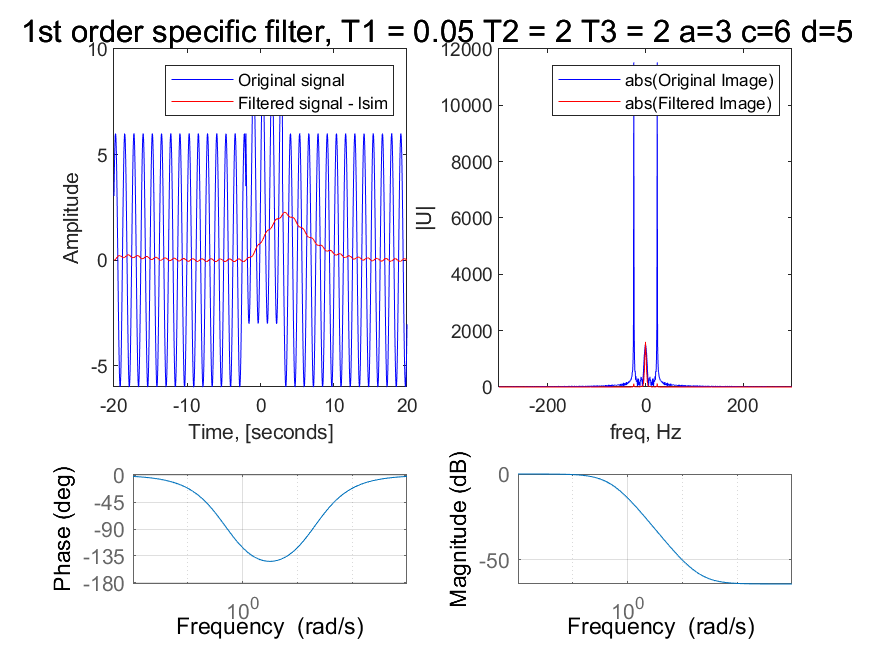
\includegraphics[width=1\textwidth]{test_specific_filter=3_b=0_c=6_d=5_T1=0_05_T2=2_00_T3=2_00.png}
	\caption{Испытание 3}
\end{figure}


\begin{figure}[ht]
    \centering
    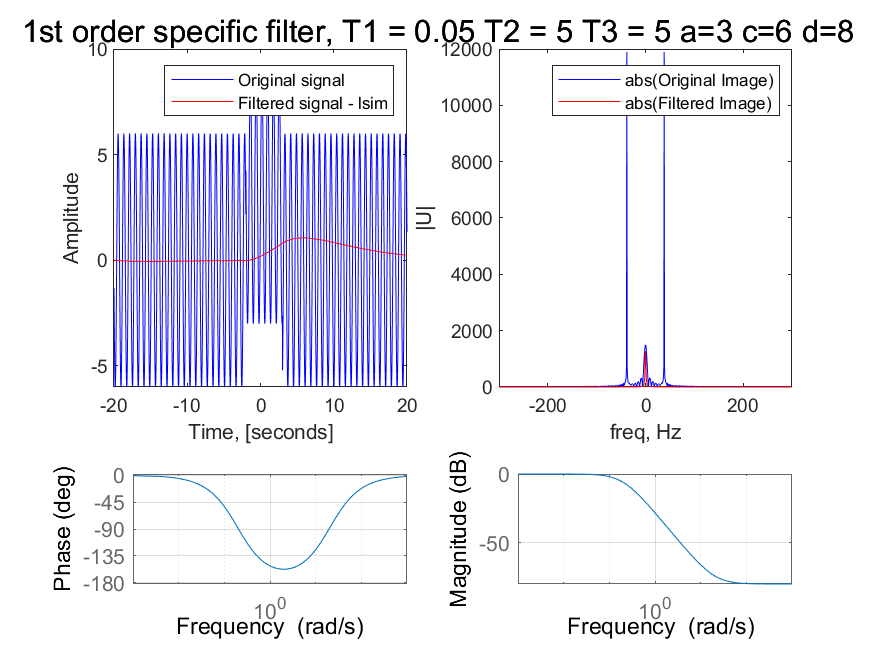
\includegraphics[width=1\textwidth]{test_specific_filter=3_b=0_c=6_d=8_T1=0_05_T2=5_00_T3=5_00.png}
	\caption{Испытание 4}
\end{figure}


\newpage
\newpage
\subsection{Выводы}
Чисто эмпирическим путём удалось выяснить, что похоже, равенство $T_2=T_3$ - даёт очень хорошие результаты. Также при этом $T_1$ должен быть меньше двух остальных коэффциентов, и не сллишком равен им... Поэтому все испытания проводились примерно с таким соотношением.

При большом $c$ мы получаем гармонический шум с большой амплитудой, коэффициенты фильтрации для которого подбираются на глаз куда сложнее, нежели для амплитуд небольших. То же самое было и с параметром $d$, но дело не в этом. 
При небольшом $c$ результат фильтрации выходит самым гладким и точным, 
а при увелечении потери от оригинала как будто значительно увеличиваются.


\endinput